\documentclass[]{elsarticle}

%% Packages
%% Packages
% Language
\usepackage[spanish]{babel}
\usepackage[utf8]{inputenc}

\usepackage[none]{hyphenat}
\sloppy

% Page dimensions
\usepackage{geometry}

% Line numbers
\usepackage{lineno}

% Graphics
\usepackage{float}
\usepackage{graphicx}
\usepackage{subcaption}

% Mathematics
\usepackage{amsmath}
\usepackage{amsfonts}
\usepackage{amssymb}
\usepackage{mathrsfs}
\usepackage{harpoon}

\usepackage{bm}
\usepackage{mathtools}
\usepackage{physics}

\usepackage{array}

\newcolumntype{C}{>{$}c<{$}}

% Tables
\usepackage{booktabs}
\usepackage{multirow}

% Colors
\usepackage{xcolor}

% Things to do
\usepackage{todonotes}

% Expected value
\DeclareMathOperator{\E}{\mathbb{E}}

\usepackage[makeroom]{cancel}

% Section formatting
\usepackage{titlesec}
\titlelabel{\thetitle\quad}

% Elsevier article
\usepackage{etoolbox}

\patchcmd{\abstract}{Abstract}{Resumen}{}{}
\patchcmd{\keyword}{Keywords}{Palabras clave}{}{}

%% Journal
\journal{Ingeniería y Ciencia}

\begin{document}

\begin{frontmatter}

%% Title, authors and addresses
\title{Diferencias Finitas para la Valoración de Opciones}

\author{Sarah Henao Gallego}
\ead{shenaog@eafit.edu.co}

\author{Santiago Hincapié Potes}
\ead{shinca12@eafit.edu.co}

\author{Luisa Fernanda Londoño Montoya}
\ead{llondo61@eafit.edu.co}

\address{Universidad EAFIT, Medellín--Colombia.}

%% Abstract here
\begin{abstract}
\end{abstract}

%% In the form: keyword \sep keyword
\begin{keyword}
\end{keyword}

\end{frontmatter}

\section{Introducción}
\label{sec:intro}
\input{sections/intro}

\section{Contexto}
\label{sec:context}
\input{sections/context}

\section{Análisis cualitativo}
\label{sec:qualitative_an}
\input{sections/qualitative_an}

\section{Análisis cuantitativo}
\label{sec:quantitative_an}
\input{sections/quantitative_an}

% Carreta 1 -- Retornos + Histograma

Los retornos instantáneous fueron calculados con la siguiente ecuación: 
\begin{align}
R_{t_i} = \frac{S_{t_i}-S_{t_i-1}}{S_{t_i-1}}
\end{align}
Con esta construcción, podemos asegurar que los retornos instantáneos siguen una distribución normal, como visto en el histograma de la Figure \ref{fig:histograma}. 

% Figure 1 -- Retornos + Histogram
\begin{figure}
  \centering
  \begin{subfigure}[ht]{\textwidth}
    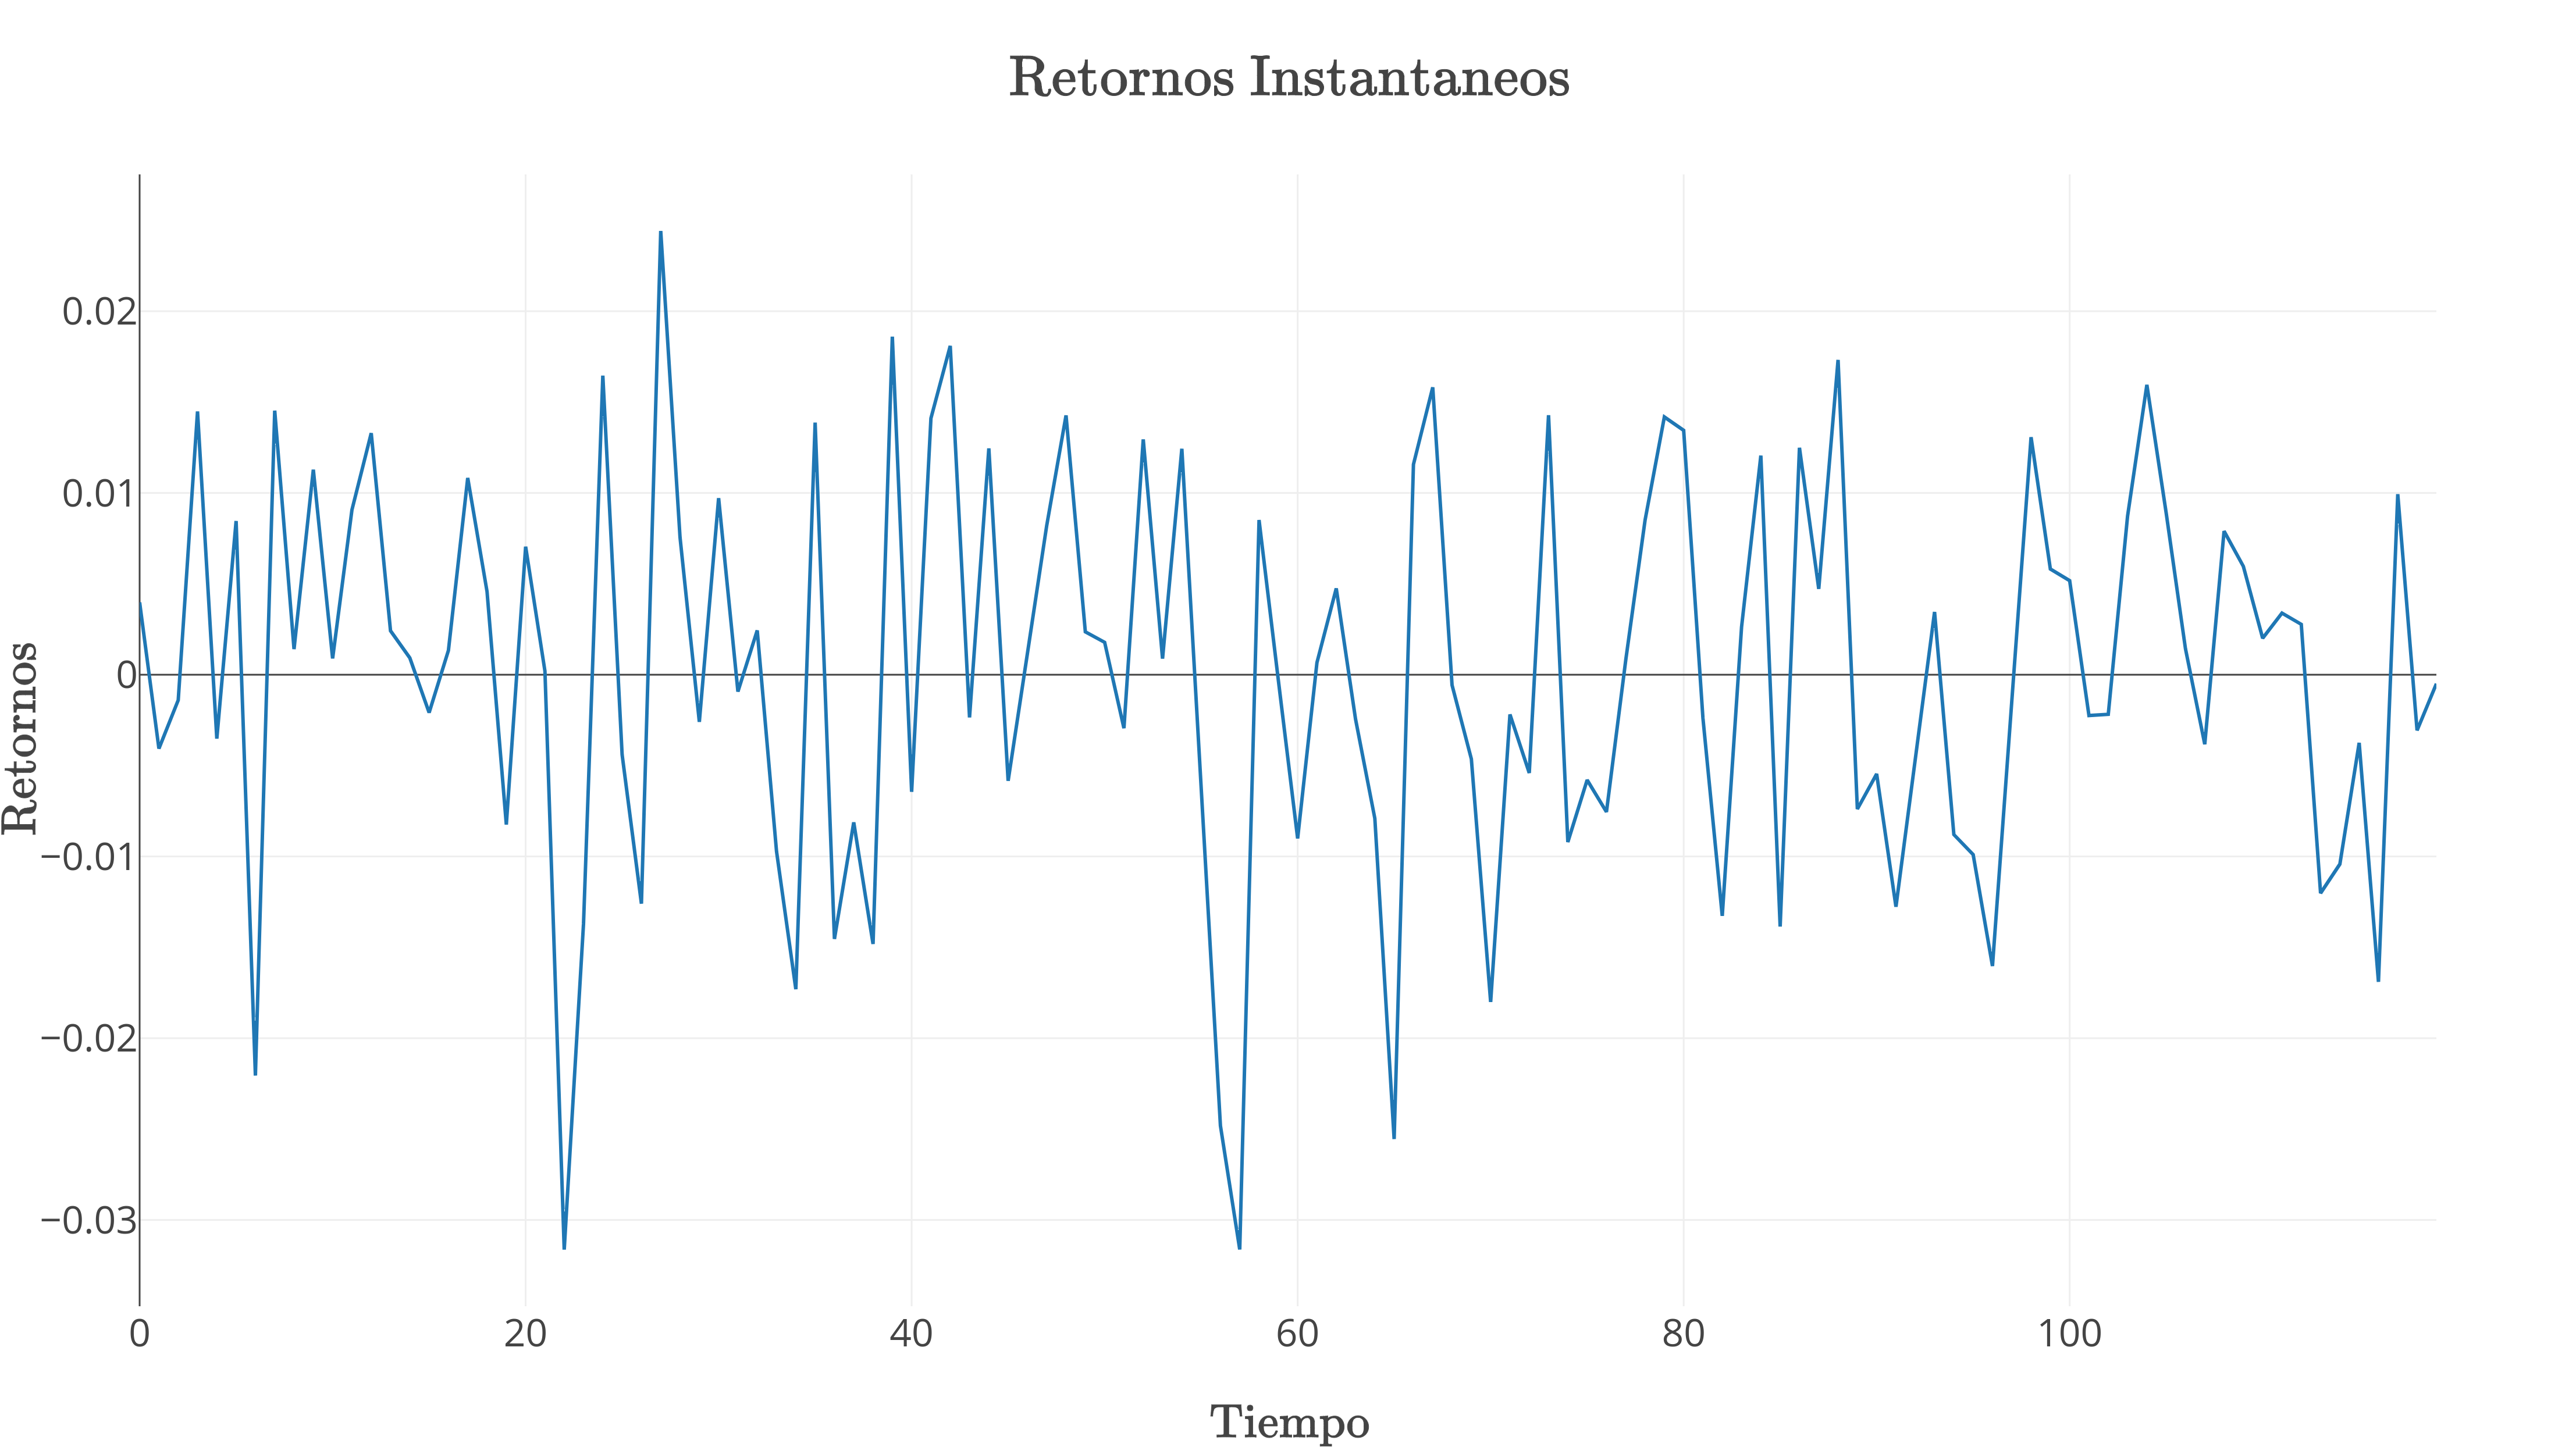
\includegraphics[width=\textwidth]{noise.png}
    \caption{Retornos Instantáneos. Los retornos instantáneos describen los cambios en el precio de la acción con respecto al día anterior y se calcularón como $R_{t_i} = \frac{S_{t_i}-S_{t_i-1}}{S_{t_i-1}}$.  }
    \label{fig:retornos}
  \end{subfigure}
  
    \begin{subfigure}[ht]{\textwidth}
      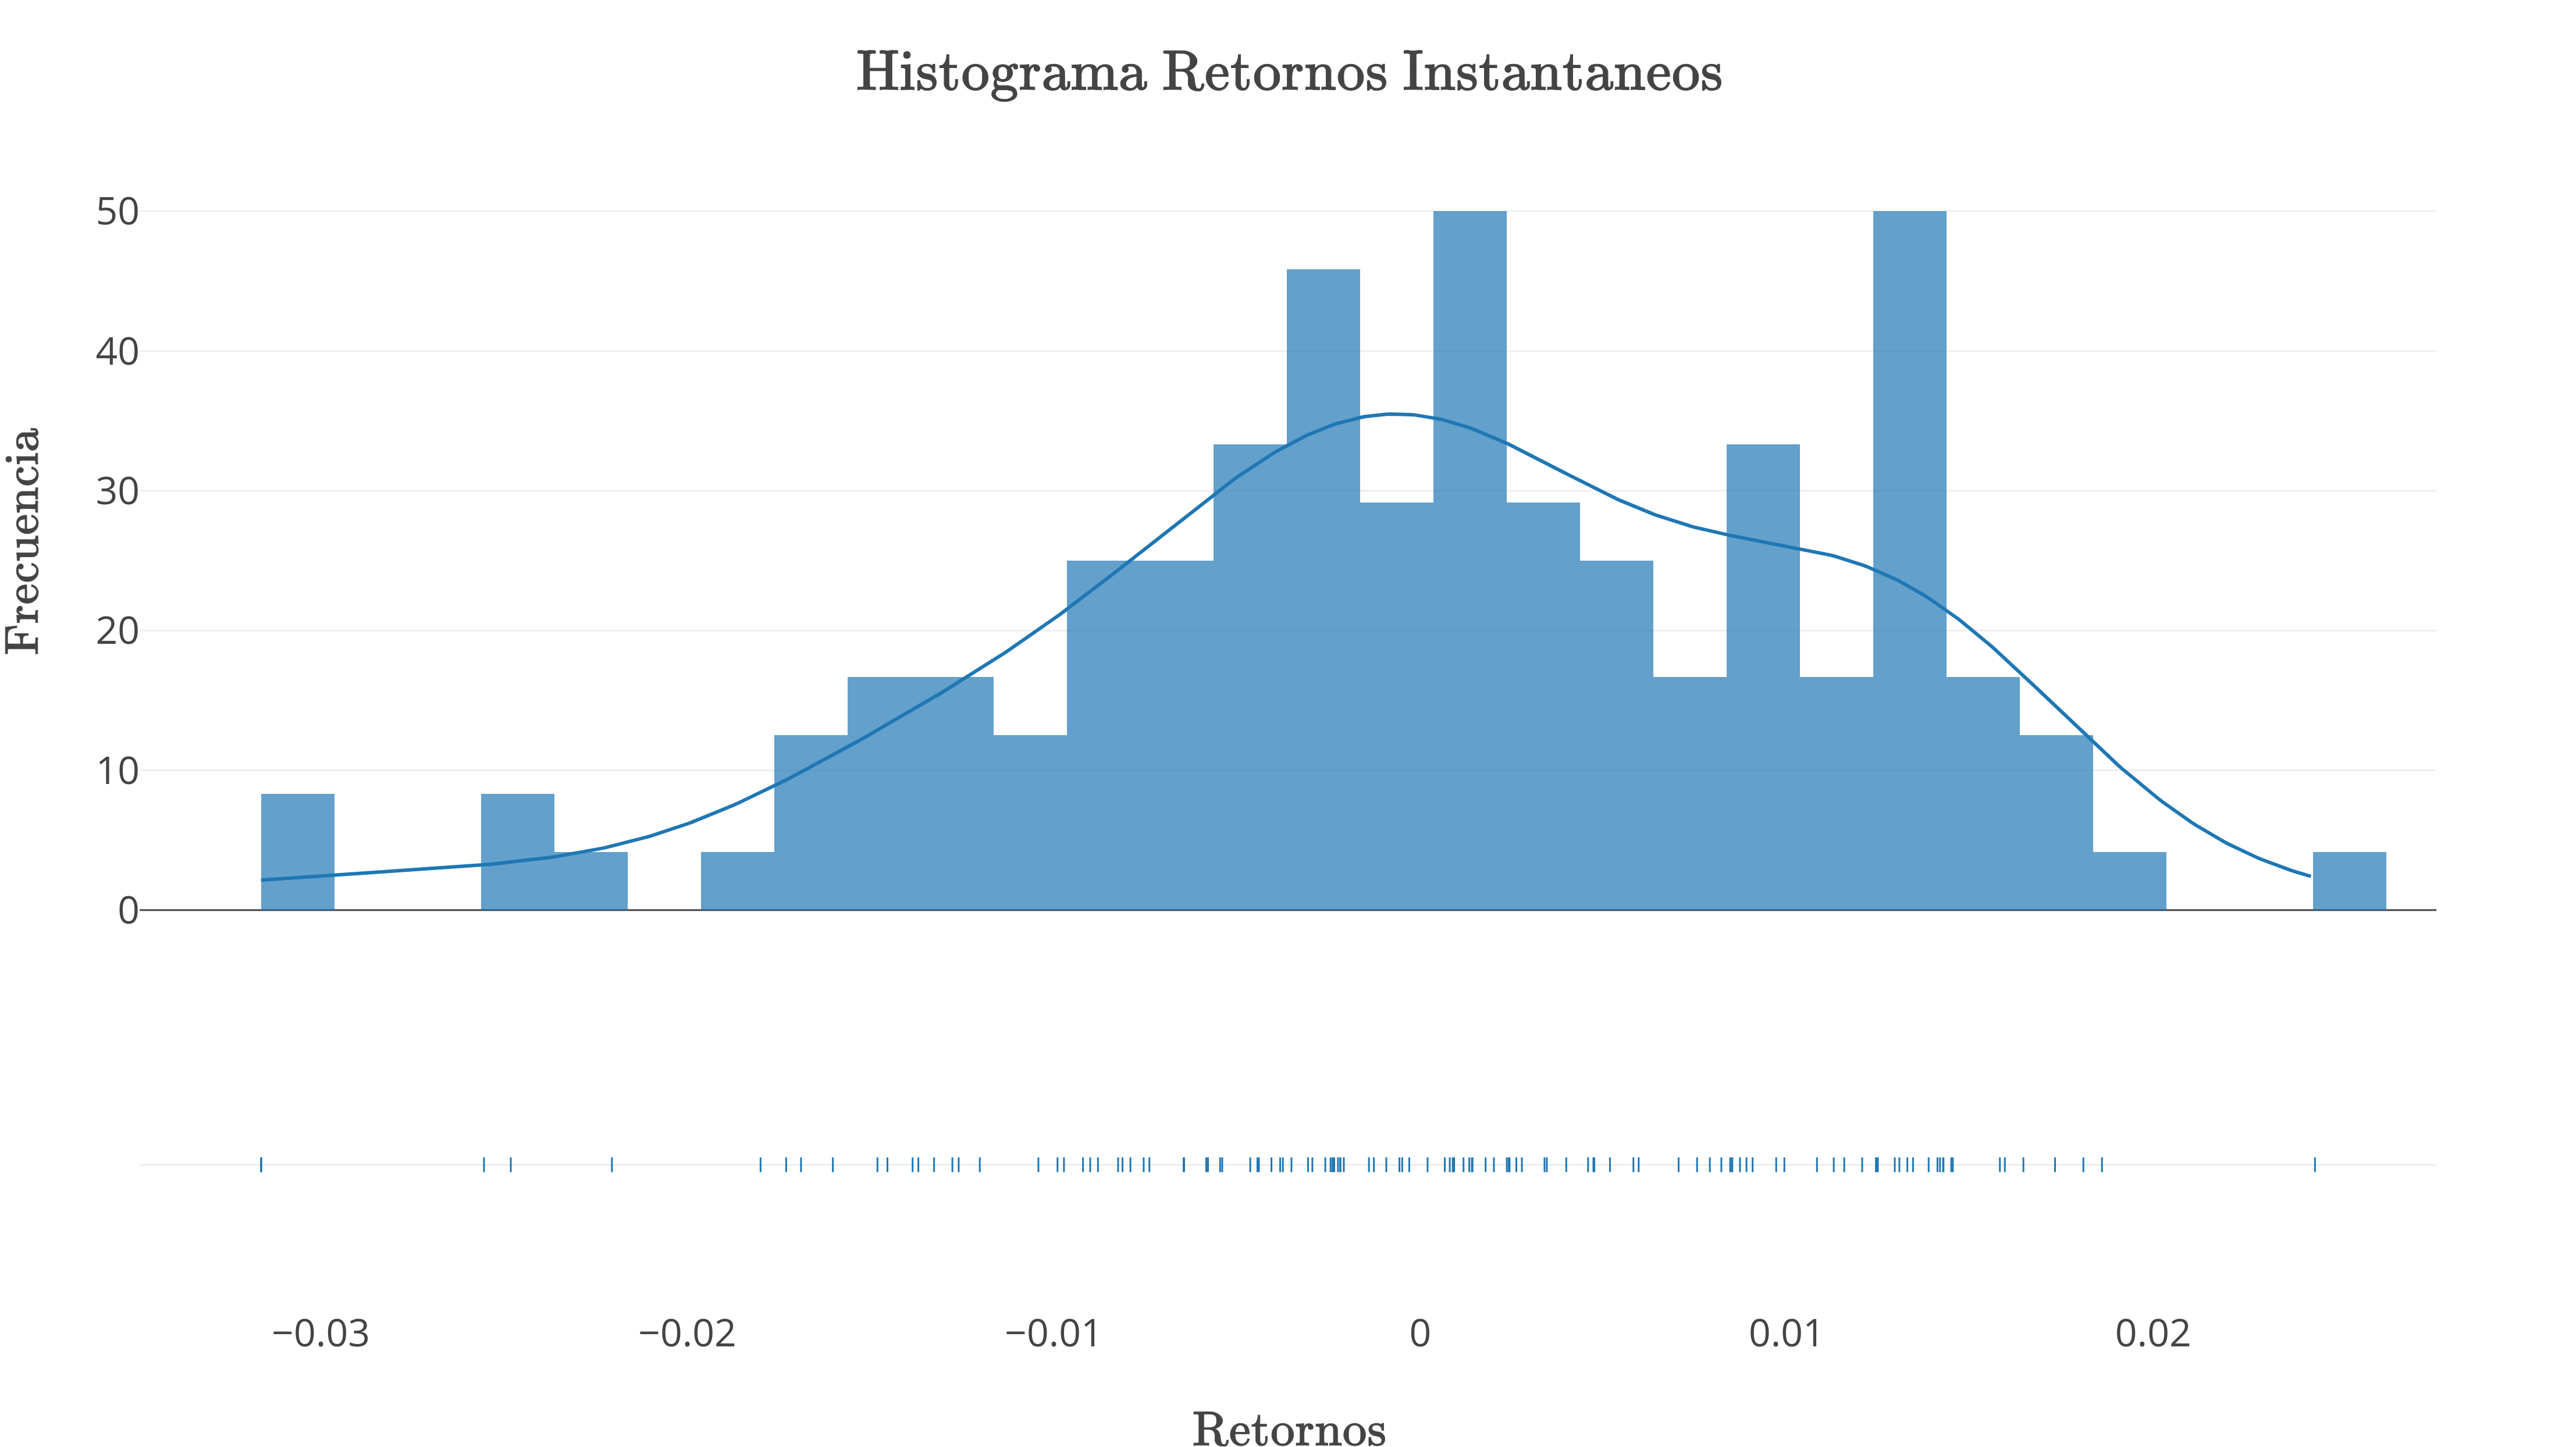
\includegraphics[width=\textwidth]{hist.png}
      \caption{Histograma de los retornos instantáneos. Los retornos instantáneos, en el intervalo de tiempo desde Mayo 9 de 2017 a Octubre 26 de 2017, siguen una distribución normal con media TAN y varianza TAN.}
      \label{fig:histograma}
    \end{subfigure}
    \caption{Los retornos instantáneous de Amazon.com, Inc. en el periodo de tiempo Mayo 9 de 2017 a Octubre 26 de 2017. Base de datos tomado por REF-NASDAQ-AMZN }\label{fig:retornosyhistograma}
  \end{figure}

% Carreta 2 -- Estimando Sigma 
Ahora, para estimar la varianza de los datos $\sigma$, se usará la formula: 
\begin{align}
	\hat{\sigma} = \sqrt{\frac{Var(R_{t_i})}{\Delta t_i}}
\end{align}



\section{Diferencias finitas}
\label{sec:bin_tree}
\input{sections/finite_diff}

\section{Diferencias finitas aplicadas a la Valoración de opciones}
\label{sec:pricing}
\input{sections/pricing}

\section{Resultados experimentales}
\label{sec:results}
\input{sections/results}

% Carreta Resultados 1 -- Convergencia 
En la Figure \ref{fig:convergencia}, podemos ver una comparación entre la solución teórica de la ecuación de Black Scholes y las aproximaciónes via el método de diferencias finitas. Aquí $dS$ denota los cambios en el precio de la acción subyacente entre $t$ y $t + dt$. A medida que el $dS \rightarrow 0$, obtenemos soluciones númericas más cercanas a la solución teórica. 

% Figure 1 -- Convergencia
\begin{figure}[ht]
\centering
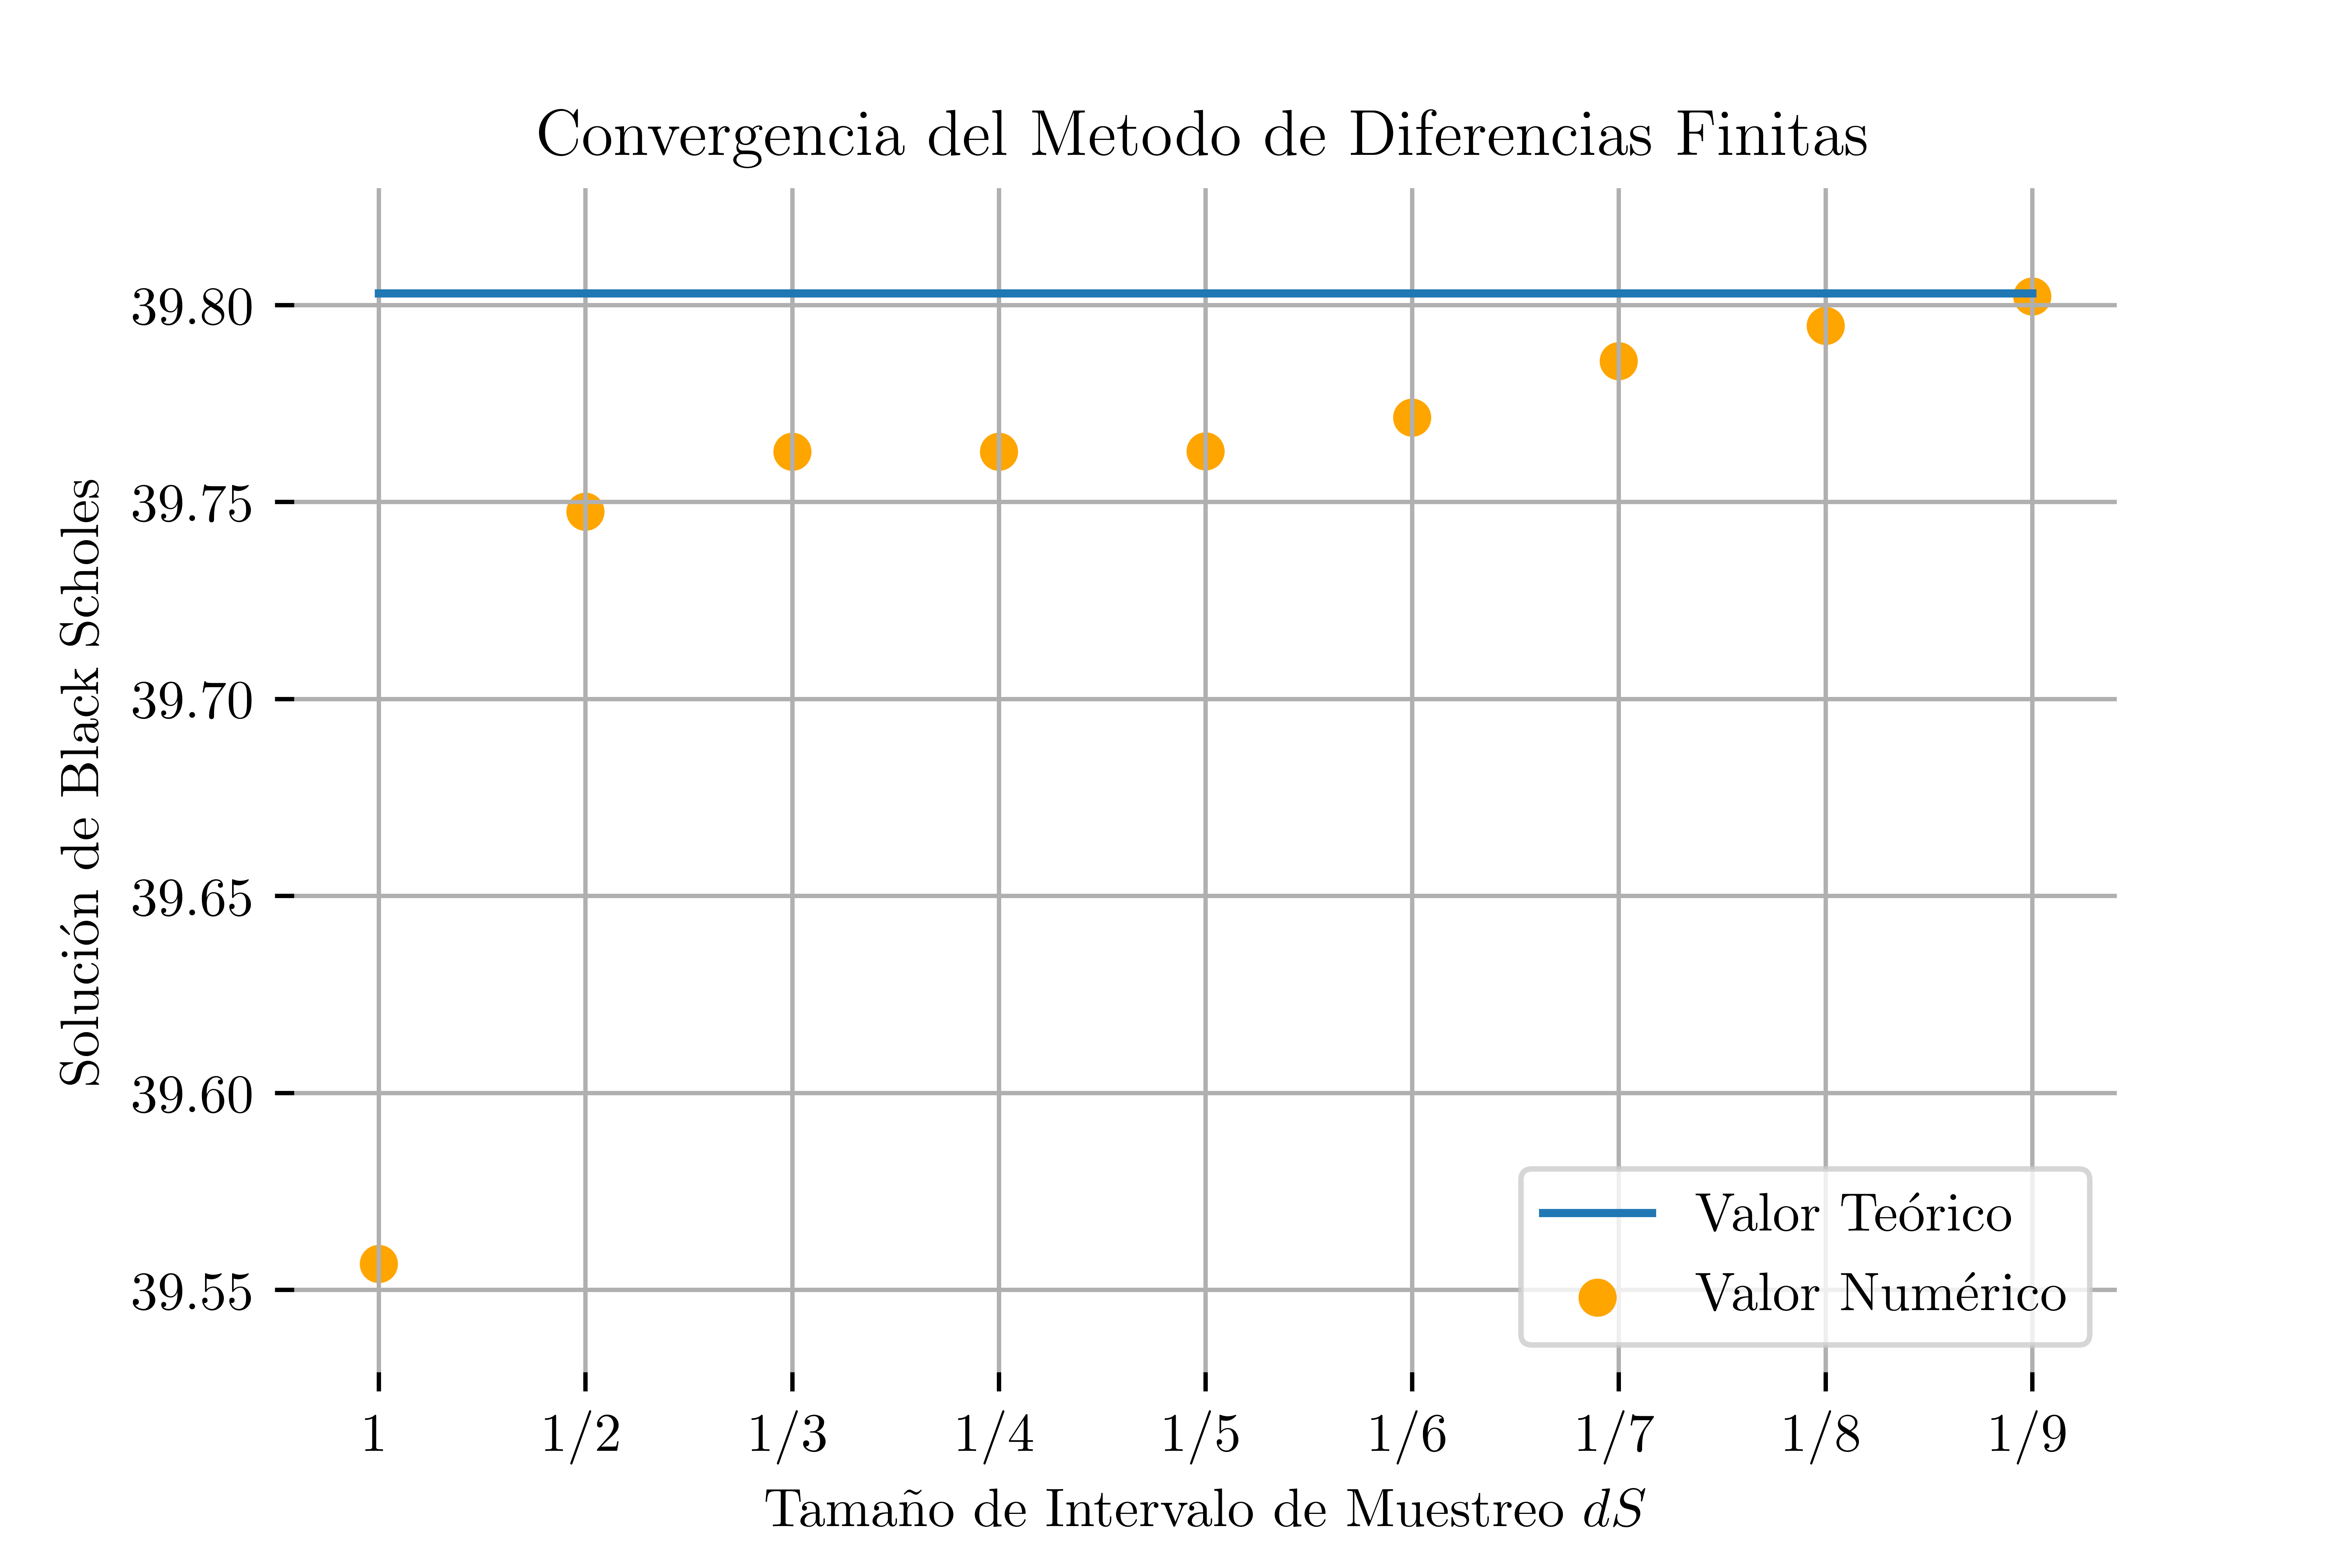
\includegraphics[width=\textwidth]{error.png}
\caption{Comparación entre diferentes soluciónes númericas a la ecuación de Black Scholes via el método de diferencias finitas con la solución teórica de Black Scholes. Las diferentes soluciónes númericas se generan por variar el intervalo de muestreo $dS$.}
\label{fig:convergencia}
\end{figure}


\section{Conclusiones}
\label{sec:conclusions}
\input{sections/conclusions}

\section*{Referencias}
% \bibliographystyle{model1-num-names}
% \bibliography{sample.bib}

\section*{Anexo --- Código}
\label{sec:annex}
\input{sections/annex}

\end{document}